\subsection{Выбор средства разработки пользовательских интерфейсов}

Для разработки интерактивного пользовательского интерфейса веб приложений с помощью языка JavaScript существует множество библиотек и фреймворков (программных платформ, определяющих структуру системы и позволяющих облегчить разработку). Наиболее популярными из них являются~\cite{stateofjs}:

\begin{enumerate}
  \item React;
  \item Angular;
  \item Vue;
  \item Svelte;
  \item Preact
  \item Ember.
\end{enumerate}

На рисунке~\ref{img:stateofjs__rank-usage} показана популярность фреймворков и библиотек разработки пользовательских интерфейсов~\cite{stateofjs}. Исходя из этих данных, выбор средства для разработки производился из трёх наиболее популярных: React, Angular и Vue.

\begin{figure}[H]
  \centering
  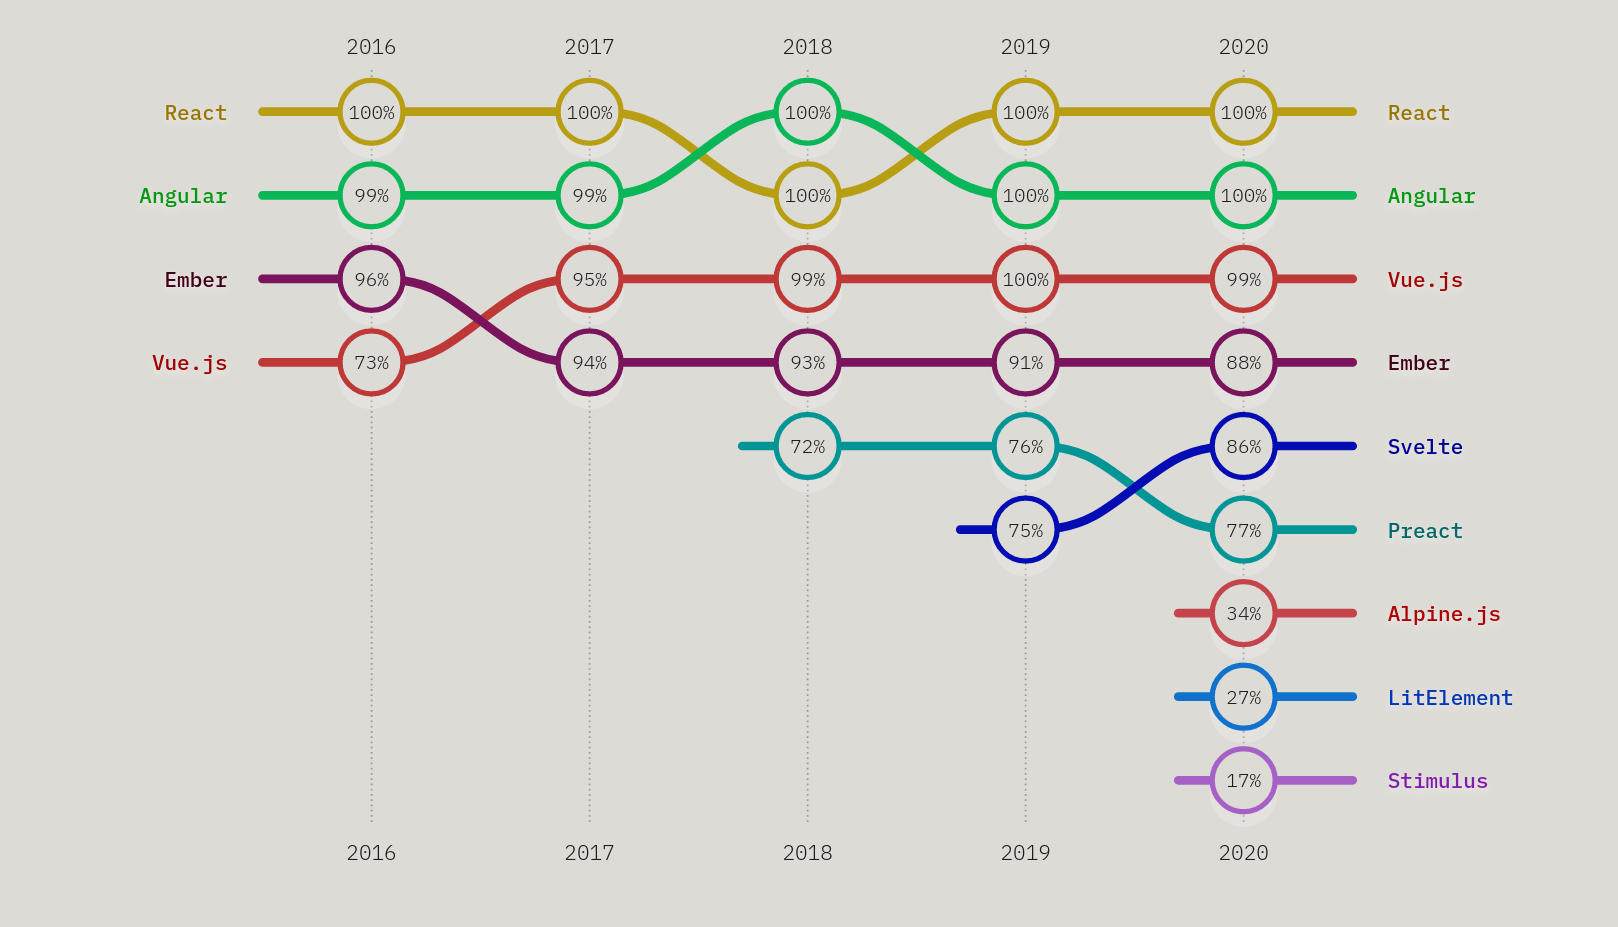
\includegraphics[width=0.9\textwidth]{assets/images/theoretical2/usageRank.png}
  \caption{Популярность фреймворков и библиотек разработки пользовательских интерфейсов}
  \label{img:stateofjs__rank-usage}
\end{figure}

Angular является фреймворком, разрабатываемым компанией Google, для создания клиентских приложений~\cite{angular}. В первую очередь, Angular подразумевается как средство для создания одностраничных приложений, или SPA приложений. В качестве основного языка программирования используется Typescript, являющийся надстройкой языка JavaScript, привносящий возможность статической типизации, а также позволяющий упростить разработку больших приложений~\cite{typescript}.

Одним из главных недостатков Angular является высокий размер пакета, около 500КБ~\cite{stateofjs}, что негативно сказывается на пользовательском опыте ввиду долгой загрузки пакета Angular по мобильной сети.

Vue является прогрессивным фреймворком для создания пользовательских интерфейсов~\cite{vue}. Vue является пригодным для постепенного внедрения. Его ядро в первую очередь решает задачи уровня представления, что упрощает интеграцию с другими библиотеками и существующими проектами. С помощью Vue можно разрабатывать одностраничные приложения, или SPA, если использовать его совместно с современными инструментами и дополнительными библиотеками.

Хотя и Vue поддерживает масштабируемость, на практике это добиться крайне сложно, так как для этого необходимо использовать дополнительными библиотеками Vue и миксинами~\cite{vue}.

React является JavaScript-библиотекой для создания пользовательских интерфейсов, разрабатываемой компанией Facebook~\cite{react}. С помощью React можно разрабатывать одностраничные приложения, или SPA, используя JSX (подобный HTML синтаксис) для шаблонов. Также в качестве разработки можно выбрать язык TypeScript.

Ввиду того, что React не является фреймворком, при разработке можно использовать только необходимый функционал React, не нагружая проект дополнительными неиспользуемыми модулями~\cite{react}.

Ввиду своей популярности и преимущества в виде гибкости использования, для разработки пользовательского интерфейса был выбрал React.